\documentclass{article}
\usepackage{tabto}
\usepackage{graphicx}
\usepackage[utf8]{vietnam}
\usepackage{url}
\usepackage[figurename=Fig.]{caption}
\renewcommand{\figurename}{Fig.}
\usepackage{caption}
\usepackage[english]{babel}

\addto\captionsenglish{% Replace "english" with the language you use
  \renewcommand{\contentsname}%
    {Content}%
}
\title{\textbf{MaSSP AI PROJECT TECHNICAL REPORT}}
\author{Team 3:\\
Nìm Trí Nghĩa - Hồ Chí Vương - Nguyễn Khắc Minh}
\date{Monday, July 8th, 2019}



\begin{document}
\maketitle
\newpage
\tableofcontents
\newpage
\textit{Project theme: OBJECT DETECTION – Finding certain objects from input images or videos} 
\graphicspath{ {./images/} }

\section{Introduction}
\tab This report will be dedicated to our final product: how to use it, how it works and our future plan with it\\
Here are a couple of things that we will not include or assume that you are familiar with:
\begin{itemize}
	\item CNN and similar neural networks (except Yolo)
	\item the math between layers (that includes back-propagation and functions such as softmax)
	\item PCA
	
\end{itemize}


\section{Our final application}
The final product we produced can be viewed and tested here: \url{https://github.com/goodudetheboy/MaSSP-Team3.git}

\section{Description}
\tab This is an app for finding lost items in real-time, simply run the application, choose an item from our item list and click the "Let's find your stuff" button. It will take roughly 10s for it to run and depending on your system, detect your item! (For reference, a 1050ti can output around 15-20 fps)

\newpage
\subsection{Demo}
\begin{figure}[h!]
	\centerline{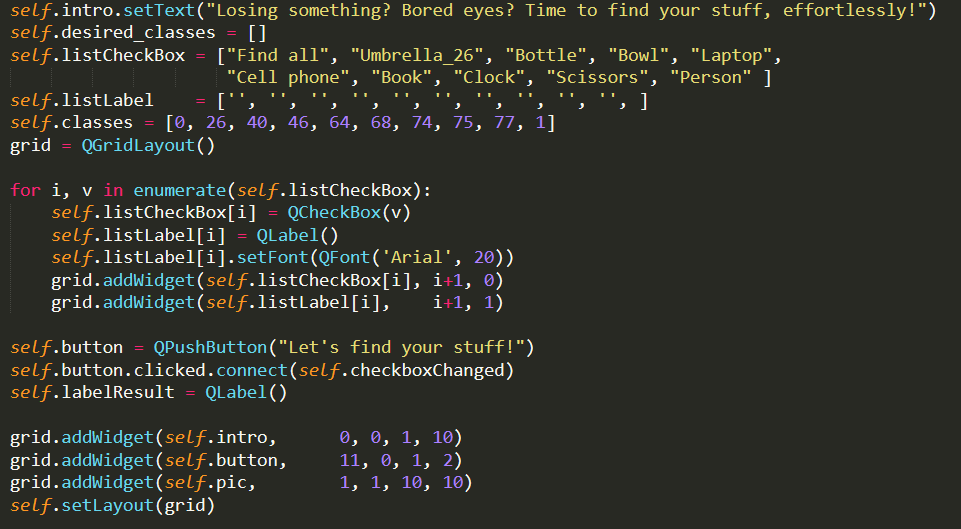
\includegraphics[scale=0.7]{demo.PNG}}
	\caption*{Image 1: a screenshot of live camera detection}
\end{figure}


\subsection{How we trained our model}
\tab We used the Detection system \textbf{Yolov3} and dataset from \textbf{the Cocodataset} to train our model. The results were that the model is extremely sensitive to new images and can detect items with moderate accuracy most of the time. However, due to how the system work, the bigger the item, the harder it is for it to detect.\\
Should you want your program to detect even more sensitively, you can trade off a bit of your accuracy but for more results by decreasing the IoU and score variables in the \textbf{$reading_video.py$} file.

\section{Unified framework (TEFPA)}
\subsection{T - Task}
What we expect here is a model to detect objects on live-camera.
\subsection{E - Experience}
Our training data comes from \url{Cocodataset.org}.
\subsection{F - Function space}
This is derived by Yolo from our live images.
\subsection{P - Performance}
The classification of boundary boxes was tested and trained using \textbf{Sum of squared errors}
\subsection{A - Algorithm}
Our model is trained using the multi object detector Yolo.

\section{Yolo}
Yolo is very much like a typical CNN, its structure is similar and could be confused with R-CNN. However, where CNN goes from regions to regions to try and extract basis functions from a given function space, Yolo does this simultaneously. That is, it employs a different method to extract information.\\
It follows these steps:
\begin{itemize}
	\item First, it divides an image into smaller squares with equal area (13x13, 14x18 for example)
	\begin{figure}[h]
		\centerline{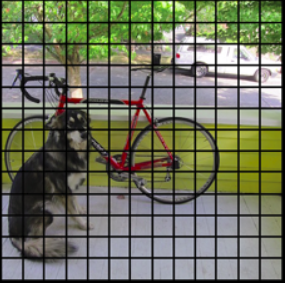
\includegraphics[scale=1]{1.PNG}}
		\caption*{Image 2: gridding the image}
	\end{figure}
	\item these square simultaneously extract features (using PCA) and make predictions for the appropriate size of anchor boxes within. These boxes can be thought of as clusters of points in a vector space. Their size gets more and more fit with the object within (or sometimes bigger than) the grid.
	\begin{figure}[h]
		\centerline{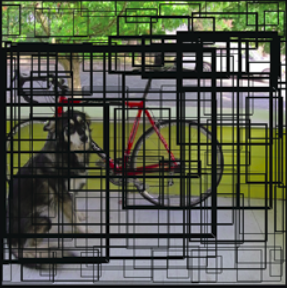
\includegraphics[scale=1]{2.PNG}}
		\caption*{Image 3: Creating anchor boxes}
	\end{figure}
	\item After choosing the best boxes, each grid will make a prediction of what the item within the box may be. This is where we will be comparing our predictions with our ground truth (dataset).
	\item To get a geometric idea of what this looks like, imagine each prediction is a probability vector inside a vector space. This vector space contains clusters of points, and each of these clusters comprises our already defined and comparable ground truths. The algorithm will predict the dimension with the highest probability, meaning it is closest to that corresponding area (cluster).
	\begin{figure}[h]
		\centerline{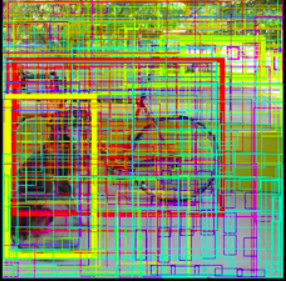
\includegraphics[scale=1]{3.PNG}}
		\caption*{Image 4: Classification}
	\end{figure}	 
	\item finally, the \textbf{IoU} parameter comes into play. If there is no value higher than our \textbf{IoU} in that vector then that prediction will be discarded, leaving only ones that the program is sure of and those we have properly trained and defined.
	\begin{figure}[h]
		\centerline{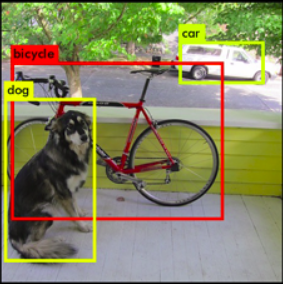
\includegraphics[scale=1]{4.PNG}}
		\caption*{Image 5: Final result}
	\end{figure}
\end{itemize}

\section{future plans}
\tab This is a new experience for all of us within the team and it goes without saying that we learned a lot and have definitely grown as well. Since we currently have no plan or project we will hopefully use this experience as the foundation for future prospects after we have departed from each other.\\
We got this opportunity thanks to MaSSP, a summer program that we have definitely not regretted a single second of. We would like a special thanks to our mentors: Hưng, Giang, Bảo, Tùng, Hiếu... as well as friends that we made during our summer camp here in Ha Noi.

\section{bibliograhy}
\tab $[1]$Hollemans, M. (2017, May 20). Real-time object detection with YOLO. Retrieved July 12, 2019, from \url{https://machinethink.net/blog/object-detection-with-yolo/}\\
\tab $[2]$Redmon, J. (2018). YOLOv3: An Incremental Improvement. Retrieved July 12, 2019, from \url{https://pjreddie.com/darknet/yolo/}\\
\tab $[3]$Chablani, M., \& Chablani, M. (2017, August 21). YOLO - You only look once, real time object detection explained. Retrieved July 12, 2019, from \url{https://towardsdatascience.com/yolo-you-only-look-once-real-time-object-detection-explained-492dc9230006}


\end{document}		


\end{document}